\documentclass[11pt]{article}

% Use "final" for the camera-ready version.
% Change to "preprint" to generate a non-anonymous version with page numbers.
\usepackage[final]{acl}

% Standard package includes
\usepackage{times}
\usepackage{latexsym}
\usepackage{amsmath, amssymb, amsthm}
\usepackage{booktabs}
\usepackage{algorithm}
\usepackage{algpseudocode}
\usepackage{multirow}
\newtheorem{theorem}{Theorem}
\newtheorem{proposition}{Proposition}
\newtheorem{lemma}{Lemma}
\newcommand{\stderr}[1]{\ensuremath{{\scriptstyle\pm}{\scriptstyle #1}}}

% For proper rendering and hyphenation of words containing Latin characters (including in bib files)
\usepackage[T1]{fontenc}
% For Vietnamese characters
% \usepackage[T5]{fontenc}
% See https://www.latex-project.org/help/documentation/encguide.pdf for other character sets

% This assumes your files are encoded as UTF8
\usepackage[utf8]{inputenc}

% This is not strictly necessary, and may be commented out,
% but it will improve the layout of the manuscript,
% and will typically save some space.
\usepackage{microtype}

% This is also not strictly necessary, and may be commented out.
% However, it will improve the aesthetics of text in
% the typewriter font.
\usepackage{inconsolata}

%Including images in your LaTeX document requires adding
%additional package(s)
\usepackage{graphicx}

% If the title and author information does not fit in the area allocated, uncomment the following
%
%\setlength\titlebox{<dim>}
%
% and set <dim> to something 5cm or larger.

\title{K-FORGE: Fisher-Guided Initialization for Preference-Based LLM Unlearning}

% Author information can be set in various styles:
% For several authors from the same institution:
% \author{Author 1 \and ... \and Author n \\
%         Address line \\ ... \\ Address line}
% if the names do not fit well on one line use
%         Author 1 \\ {\bf Author 2} \\ ... \\ {\bf Author n} \\
% For authors from different institutions:
% \author{Author 1 \\ Address line \\  ... \\ Address line
%         \And  ... \And
%         Author n \\ Address line \\ ... \\ Address line}
% To start a separate ``row'' of authors use \AND, as in
% \author{Author 1 \\ Address line \\  ... \\ Address line
%         \AND
%         Author 2 \\ Address line \\ ... \\ Address line \And
%         Author 3 \\ Address line \\ ... \\ Address line}

\author{First Author \\
  Affiliation / Address line 1 \\
  Affiliation / Address line 2 \\
  Affiliation / Address line 3 \\
  \texttt{email@domain} \\\And
  Second Author \\
  Affiliation / Address line 1 \\
  Affiliation / Address line 2 \\
  Affiliation / Address line 3 \\
  \texttt{email@domain} \\}

%\author{
%  \textbf{First Author\textsuperscript{1}},
%  \textbf{Second Author\textsuperscript{1,2}},
%  \textbf{Third T. Author\textsuperscript{1}},
%  \textbf{Fourth Author\textsuperscript{1}},
%\\
%  \textbf{Fifth Author\textsuperscript{1,2}},
%  \textbf{Sixth Author\textsuperscript{1}},
%  \textbf{Seventh Author\textsuperscript{1}},
%  \textbf{Eighth Author \textsuperscript{1,2,3,4}},
%\\
%  \textbf{Ninth Author\textsuperscript{1}},
%  \textbf{Tenth Author\textsuperscript{1}},
%  \textbf{Eleventh E. Author\textsuperscript{1,2,3,4,5}},
%  \textbf{Twelfth Author\textsuperscript{1}},
%\\
%  \textbf{Thirteenth Author\textsuperscript{3}},
%  \textbf{Fourteenth F. Author\textsuperscript{2,4}},
%  \textbf{Fifteenth Author\textsuperscript{1}},
%  \textbf{Sixteenth Author\textsuperscript{1}},
%\\
%  \textbf{Seventeenth S. Author\textsuperscript{4,5}},
%  \textbf{Eighteenth Author\textsuperscript{3,4}},
%  \textbf{Nineteenth N. Author\textsuperscript{2,5}},
%  \textbf{Twentieth Author\textsuperscript{1}}
%\\
%\\
%  \textsuperscript{1}Affiliation 1,
%  \textsuperscript{2}Affiliation 2,
%  \textsuperscript{3}Affiliation 3,
%  \textsuperscript{4}Affiliation 4,
%  \textsuperscript{5}Affiliation 5
%\\
%  \small{
%    \textbf{Correspondence:} \href{mailto:email@domain}{email@domain}
%  }
%}

\begin{document}
\maketitle
\begin{abstract}
Preference-based LLM unlearning methods such as NPO and SimNPO must discover directions that suppress forget-set behavior without damaging retained capability. We ask whether a second-order initializer can supply such a direction before iterative optimization begins. K-FORGE uses forget- and retain-set Fisher information to construct a retain-aware low-rank edit, then starts NPO or SimNPO from the edited checkpoint. On TOFU with Llama-3.2-1B, the one-shot edit gives a controllable forget--utility frontier. In a three-seed wall- and FLOP-matched NPO rerun, K-FORGE reduces Forget Q/A Probability by 22.3\% while improving utility; SimNPO retains a smaller descriptive probability gain at a slight utility cost. Four-seed Gemma-3-1B experiments preserve the primary direction, while Llama matched controls show that an arbitrary low-rank displacement does not generally reproduce the result. MUSE transfer is metric-dependent, and relearning shows no recovery defense. These results delimit K-FORGE as a curvature-aware optimization initializer rather than a standalone unlearning or robustness guarantee.
\end{abstract}

\section{Introduction}

LLM unlearning seeks to remove behavior attributable to specified training data without retraining from scratch~\citep{tofu,rmu,muse}. Iterative preference-based methods such as NPO~\citep{npo} and SimNPO~\citep{simnpo} repeatedly optimize a one-sided preference objective. Representation methods such as RMU~\citep{rmu} instead redirect intermediate activations. Structured alternatives include diagonal-Fisher dampening~\citep{foster24}, Fisher-weighted LoRA initialization~\citep{fila}, and few-step Kronecker-factored Gauss--Newton updates~\citep{kfade}.

The central difference is adaptivity. An iterative method can revise its direction after each update, whereas a one-shot method commits to one local surrogate before observing the resulting model behavior. In the reported one-shot sweep, increasing strength reduces forget probability while progressively spending utility. We therefore ask whether a closed-form edit is more useful as the starting direction for iterative unlearning than as the final unlearned model.

We answer this question by treating Kronecker-Fisher edits as initializers rather than finished unlearning procedures. We combine K-FAC-style layerwise Fisher factors~\citep{martens2015optimizing} with Fisher-weighted low-rank factorization~\citep{chekalina_2026_gfwsvd}. We estimate one factor pair on forget data and one on retain data, simultaneously diagonalize the pairs, and derive a retain-aware Wiener edit in that basis. We call the resulting construction \textbf{K-FORGE} (\textbf{K}ronecker-\textbf{F}isher \textbf{O}ne-shot \textbf{R}ank-r \textbf{G}eneralized \textbf{E}rasure).

Our experiments support this initializer view. On TOFU \texttt{forget10} with Llama-3.2-1B-Instruct, one-shot K-FORGE traces a controllable forget--utility frontier but does not replace iterative unlearning. As an initializer, it improves the early Forget Q/A Probability trajectory of NPO and SimNPO. After charging the complete setup in both wall-clock time and FLOPs, the NPO gain remains strong; SimNPO keeps a smaller probability gain with a slight utility trade-off. Llama initialization controls show that the effect is not generally reproduced by arbitrary low-rank displacement. A fourth Gemma-3-1B seed preserves the primary direction, whereas Qwen and MUSE results are weaker or metric-dependent. These outcomes motivate a specific claim---better initialization in the tested regimes---rather than universal improvement across models, benchmarks, or forgetting metrics.

Our contributions are three-fold:
\begin{enumerate}
    \item We introduce \textbf{K-FORGE}, a closed-form Fisher-guided initializer for preference-based LLM unlearning. K-FORGE uses separate forget and retain curvature estimates to construct a low-rank edit that gives NPO and SimNPO a more informative starting point than the original checkpoint.

    \item We derive a two-Fisher Wiener formulation that makes the role of retain awareness explicit. The full-rank solution is exact, and the practical low-rank case is handled by a stated relaxation rather than by assuming an unavailable closed-form optimum.

    \item We show that K-FORGE improves the early Forget Q/A Probability trajectory of fixed NPO and SimNPO optimizers on TOFU \texttt{forget10}. The NPO gain survives direct FLOP and wall-clock matching; model-family, benchmark-transfer, and recovery audits identify both reproducible gains and the boundaries of the claim.
  \end{enumerate}
  
K-FORGE is complementary to existing unlearning methods: it changes the starting point, not the downstream preference objective. Code is available at \url{https://github.com/etomoscow/kron_unlearn}.


\section{Related Work}

\paragraph{LLM unlearning methods.}
Preference-based unlearning is the immediate setting for our work. NPO~\citep{npo} regularizes forget-set ascent through a reference-model preference term, while SimNPO~\citep{simnpo} removes the reference model. Other families change the unlearning rule itself, for example by redirecting activations as in RMU~\citep{rmu}, combining forget and retain gradients, or subtracting task vectors. K-FORGE asks an orthogonal question: with the downstream rule held fixed, can forget/retain curvature provide a better starting point? We study that question on TOFU~\citep{tofu} and MUSE~\citep{muse} through the OpenUnlearning harness~\citep{openunlearning}; we do not propose another preference loss.

\paragraph{Fisher-guided initialization and second-order unlearning.}
FILA~\citep{fila} uses relative-Fisher weighted low-rank approximation to initialize LoRA; VILA~\citep{vila} improves its estimation and efficiency; ReGLU~\citep{xiao-etal-2026-representation} combines representation-subspace initialization with an orthogonality loss. These works establish informed unlearning initialization. Other second-order methods change the update rule: SOUL~\citep{soul} uses a Sophia-style optimizer~\citep{sophia}, K-FADE~\citep{kfade} uses Kronecker-factored Gauss--Newton steps, and WIN-U~\citep{winu} uses Woodbury-scaled Newton updates. We do not claim Fisher-guided initialization itself as novel. K-FORGE instead derives a two-Fisher Kronecker Wiener edit with an exact full-rank solution and stated low-rank relaxation, folds it into the base checkpoint, and leaves NPO or SimNPO unchanged.

\paragraph{Fisher information approximations.}
K-FAC~\citep{martens2015optimizing} and EK-FAC~\citep{exfac} approximate layer-wise Fisher information with Kronecker factors, making structured curvature computations tractable. Kronecker-Fisher approximations have also been used for
influence functions at LLM scale~\citep{DBLP:journals/corr/abs-2308-03296} and for compression via matrix-free Fisher factorization and GFWSVD~\citep{chekalina_2026_gfwsvd}. K-FORGE uses K-FAC-style covariance factors and extends the Fisher-weighted low-rank construction to separate forget and retain metrics.

\begin{figure*}
    \centering
    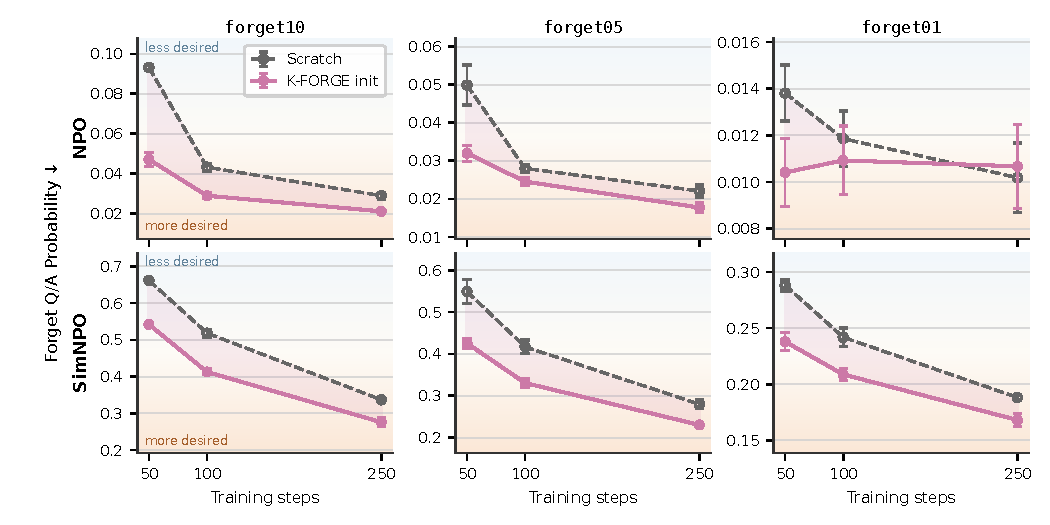
\includegraphics[width=\linewidth, trim=1cm 0.500cm 0.500cm 2cm]{open-unlearning/saves/figures/kforge_corrected/fig2_improved.pdf}
    \caption{Matched downstream-step forget-probability trajectories on TOFU. Points show three-seed means with standard-deviation bars; panels use split-specific y-axis ranges. Gains are clearest on \texttt{forget10}/\texttt{forget05} and for SimNPO; NPO on \texttt{forget01} is near the noise floor and reverses slightly at 250 steps. Additional initialization controls are reported in Tables~\ref{tab:init_controls_forget10} and~\ref{tab:transfer_controls}.}
    \label{fig:transfer_trajectories}
\end{figure*}



\section{Method}
\label{sec:method}

\subsection{Preliminaries}
\label{sec:preliminaries}

Let $\mathbf{W} \in \mathbb{R}^{n \times m}$ denote the weight matrix of a single linear layer in a pretrained model with parameters $\theta^\star$. We denote by $\mathcal{L}_f(\theta)$ and $\mathcal{L}_r(\theta)$ the expected losses on a forget set $\mathcal{D}_f$ and a retain set $\mathcal{D}_r$, respectively. For a loss-bearing token $t$, let $\mathbf{x}_t\in\mathbb{R}^m$ be the layer input and $\mathbf{g}_t\in\mathbb{R}^n$ the gradient with respect to its output. Because the per-token weight gradient is $\mathbf{g}_t\mathbf{x}_t^\top$, we use the K-FAC approximation~\citep{martens2015optimizing}
\begin{equation}
\begin{aligned}
    \mathcal{I}_F(\mathbf{W}) &\approx \mathbf{A} \otimes \mathbf{B}, \\
    \mathbf{A}&=\frac{1}{N}\sum_{t=1}^N\mathbf{x}_t\mathbf{x}_t^\top, \\
    \mathbf{B}&=\frac{1}{N}\sum_{t=1}^N\mathbf{g}_t\mathbf{g}_t^\top.
\end{aligned}
\end{equation}
We stream these covariances without materializing the $(mn)\times(mn)$ Fisher and mask padding, prompt, and other non-loss tokens. For $N$ retained token rows, factor accumulation costs $\mathcal{O}(N(m^2+n^2))$ operations and $\mathcal{O}(m^2+n^2)$ memory; the subsequent dense factorizations cost $\mathcal{O}(m^3+n^3)$. We therefore evaluate and report the one-layer setup cost directly rather than extrapolating broad many-layer scaling.

In this work, we estimate the factors twice per layer: once on $\mathcal{D}_f$ to obtain $\mathbf{A}_f, \mathbf{B}_f$, and once on $\mathcal{D}_r$ to obtain $\mathbf{A}_r, \mathbf{B}_r$. Each $d\times d$ factor $\mathbf{C}$ is symmetrized and trace-scale damped as $\mathbf{C}\leftarrow\mathbf{C}+\varepsilon\max(\operatorname{tr}(\mathbf{C})/d,10^{-12})\mathbf{I}$ before Cholesky factorization:
\begin{equation}
    \mathbf{A} = \mathbf{L}_A \mathbf{L}_A^\top, \qquad \mathbf{B} = \mathbf{L}_B \mathbf{L}_B^\top.
\end{equation}

That ensures all four factors are SPD, that the Cholesky factors $\mathbf{L}_{A_\bullet},\mathbf{L}_{B_\bullet}$ are invertible, and that $\mathbf{K}_A=\mathbf{L}_{A_r}^{-1}\mathbf{L}_{A_f}$ and $\mathbf{K}_B=\mathbf{L}_{B_r}^{-1}\mathbf{L}_{B_f}$ are non-singular. In particular $\sigma_{A,i},\sigma_{B,j}>0$ for all $(i,j)$, which we use freely in Section~\ref{sec:two_fisher_gsvd} and Appendix~\ref{sec:proofs}.

\subsection{Two-Fisher Wiener Edit}
\label{sec:two_fisher_gsvd}

Following Fisher-weighted low-rank approximation, we treat weight components with high forget-Fisher energy as directions strongly expressed on the forget distribution. We therefore shrink the post-edit weight in that metric while penalizing movement in the retain metric. This is a local design surrogate, not a guarantee that answer probability decreases; the one-shot and initialization experiments test that link empirically:
\begin{equation}
    J(\mathbf{\Delta})
    =
    \lVert \mathbf{W}+\mathbf{\Delta} \rVert^2_{F_f}
    +
    \lambda_{\mathrm{ret}}
    \lVert \mathbf{\Delta} \rVert^2_{F_r},
\label{eq:kforge_objective}
\end{equation}
where $\lVert \mathbf{X} \rVert^2_{F_\bullet}
= \operatorname{vec}(\mathbf{X})^\top
(\mathbf{A}_\bullet \otimes \mathbf{B}_\bullet)
\operatorname{vec}(\mathbf{X})$. We define cross-Cholesky maps
\begin{equation}
    \mathbf{K}_A = \mathbf{L}_{A_r}^{-1}\mathbf{L}_{A_f},
    \qquad
    \mathbf{K}_B = \mathbf{L}_{B_r}^{-1}\mathbf{L}_{B_f},
\end{equation}
with SVDs $\mathbf{K}_A = \mathbf{U}_A \mathbf{\Sigma}_A \mathbf{V}_A^\top$ and
$\mathbf{K}_B = \mathbf{U}_B \mathbf{\Sigma}_B \mathbf{V}_B^\top$. The rotated forget-whitened weight is
\begin{equation}
    \mathbf{R}
    =
    \mathbf{V}_B^\top
    \mathbf{L}_{B_f}^\top
    \mathbf{W}
    \mathbf{L}_{A_f}
    \mathbf{V}_A.
\end{equation}

Define the simultaneous diagonalizers $\mathbf{Q}_A = \mathbf{L}_{A_r}^{-\top}\mathbf{U}_A$ and $\mathbf{Q}_B = \mathbf{L}_{B_r}^{-\top}\mathbf{U}_B$, which jointly diagonalize $(\mathbf{A}_f,\mathbf{A}_r)$ and $(\mathbf{B}_f,\mathbf{B}_r)$, and let $\mathbf{H} = \mathbf{Q}_B^{-1}\mathbf{\Delta}\,\mathbf{Q}_A^{-\top}$ denote the perturbation in this basis.

\begin{theorem}[Unconstrained K-FORGE Wiener edit]
\label{thm:two_fisher_gsvd}
For $\lambda_{\mathrm{ret}}\geq 0$, the unique minimizer of Eq.~\ref{eq:kforge_objective} over $\mathbf{\Delta}\in\mathbb{R}^{n\times m}$ is
\begin{equation}
    \mathbf{\Delta}^\star
    =
    -\mathbf{L}_{B_r}^{-\top}
    \mathbf{U}_B
    (\mathbf{G} \odot \mathbf{R})
    \mathbf{U}_A^\top
    \mathbf{L}_{A_r}^{-1},
\label{eq:kforge_delta}
\end{equation}
where
\begin{equation}
    G_{ji}
    =
    \frac{\sigma_{A,i}\sigma_{B,j}}
    {\sigma_{A,i}^2\sigma_{B,j}^2+\lambda_{\mathrm{ret}}}.
\end{equation}
For $r=\min(m,n)$ the rank constraint is inactive, so $\mathbf{\Delta}^\star$ is also the rank-$r$ minimizer.
\end{theorem}

\begin{proposition}[Exact rank-$r$ solution at zero retain penalty]
\label{prop:rankr_lam0}
At $\lambda_{\mathrm{ret}}=0$, an exact rank-$r$ minimizer of Eq.~\ref{eq:kforge_objective} is obtained by the rescaling $\mathbf{Y}=\mathbf{\Sigma}_B\mathbf{H}\mathbf{\Sigma}_A$, which converts the objective into the unweighted Frobenius problem $\lVert\mathbf{Y}+\mathbf{R}\rVert_F^2$. Solving via Eckart--Young, $\mathbf{Y}_r=\operatorname{SVD}_r(-\mathbf{R})$, unscaling $\mathbf{H}_r=\mathbf{\Sigma}_B^{-1}\mathbf{Y}_r\mathbf{\Sigma}_A^{-1}$, and mapping back yields
\begin{equation}
    \mathbf{\Delta}^{\!(\!r\!)\!}_{0}\!=\!\!-\!\mathbf{L}_{B_r}^{-\top}\!\mathbf{U}_B\,\mathbf{\Sigma}_B^{-1}\operatorname{SVD}_r(\mathbf{R})\mathbf{\Sigma}_A^{-1}\,
    \!\mathbf{U}_A^\top\!\mathbf{L}_{A_r}^{-1}
\end{equation}
\end{proposition}

\paragraph{General case: separable relaxation.}
For $\lambda_{\mathrm{ret}}>0$ and $r<\min(m,n)$, the rank-$r$ problem becomes a weighted-Frobenius low-rank approximation with non-separable weights $\alpha_{ji}=\sigma_{A,i}^2\sigma_{B,j}^2+\lambda_{\mathrm{ret}}$, which is NP-hard in general~\citep{DBLP:conf/icml/SrebroJ03}. We adopt the separable relaxation that keeps the Wiener-filtered target but replaces the weights with their separable surrogate $\sigma_{A,i}^2\sigma_{B,j}^2$. Concretely,
\begin{equation}
    \widetilde{G}_{ji}
    \!=\!
    \frac{\sigma_{A,i}^2\sigma_{B,j}^2}
    {\sigma_{A,i}^2\sigma_{B,j}^2+\lambda_{\mathrm{ret}}},\!
    \quad
    \mathbf{Y}^\star
    \!=\!
    -(\!\widetilde{\mathbf{G}}\!\odot\!\mathbf{R}),
\label{eq:relaxation_target}
\end{equation}
followed by $\mathbf{Y}_r\!=\!\operatorname{SVD}_r(\mathbf{Y}^\star),\mathbf{H}_r\!=\!\mathbf{\Sigma}_B^{-1}\mathbf{Y}_r\mathbf{\Sigma}_A^{-1}$, and
\begin{equation}
    \mathbf{\Delta}^{(r)}
    \!=\!\mathbf{L}_{B_r}^{-\top}\mathbf{U}_B\,\!
    \mathbf{H}_r\,
    \mathbf{U}_A^\top\mathbf{L}_{A_r}^{-1}.
\label{eq:kforge_relaxed_delta}
\end{equation}
(The sign is absorbed into $\mathbf{Y}^\star$.)

The relaxation is exact either at full rank for any $\lambda_{\text{ret}}\ge0$, or at $\lambda_{\text{ret}}=0$ for any $r$ (Proposition~\ref{prop:limit_consistency}).

\paragraph{Interpretation.}
Let $s_{ji}=\sigma_{A,i}\sigma_{B,j}$. Then $s_{ji}^2$ is the forget-to-retain curvature ratio along coordinate $(j,i)$ of the diagonalized basis. In $\mathbf{H}$ coordinates, the exact solution scales the cancellation target by $s_{ji}^2/(s_{ji}^2+\lambda_{\mathrm{ret}})$: directions dominated by retain curvature are suppressed, while forget-dominant directions approach full cancellation. The low-rank relaxation truncates the resulting filtered target, yielding a compact initialization edit.


\paragraph{Recovering prior work.}
When all four Fisher factors are restricted to be diagonal, the simultaneous basis is coordinate-aligned up to permutations and signs, and Eq.~\ref{eq:kforge_delta} reduces to per-weight Wiener filtering of the singly-whitened weight matrix. The structure becomes close to Selective Synaptic Dampening~\citep{foster24}, but with a Wiener denominator $\sigma_{A,i}^2\sigma_{B,j}^2\!+\!\lambda_{\mathrm{ret}}$ rather than SSD's hard-clipped ratio $\min(\alpha F_f/F_r, 1)$; we use this diagonal limit as a control in Section~\ref{sec:experiments}. Setting $\mathbf{A}_r\!=\!\mathbf{I}$ and $\mathbf{B}_r\!=\!\mathbf{I}$ removes retain-set curvature awareness and yields our forget-only ablation.

\subsection{The K-FORGE Algorithm}
\label{sec:kforge_algorithm}
\begin{algorithm}[t]
\caption{K-FORGE}
\label{alg:kforge}
\begin{algorithmic}[1]
\Require Weight matrix $\mathbf{W}$, forget/retain sets $\mathcal{D}_f,\mathcal{D}_r$, rank $r$, factor damping $\varepsilon$, retain penalty $\lambda_{\mathrm{ret}}$, strength $\alpha$
\State $(\mathbf{A}_f,\mathbf{B}_f)\leftarrow \operatorname{KronFisher}(\mathbf{W},\mathcal{D}_f)$;\quad $(\mathbf{A}_r,\mathbf{B}_r)\leftarrow \operatorname{KronFisher}(\mathbf{W},\mathcal{D}_r)$
\State Trace-scale damp factors by $\varepsilon$ and compute $\mathbf{L}_{A_\bullet},\mathbf{L}_{B_\bullet}$
\State $\mathbf{K}_A\leftarrow\mathbf{L}_{A_r}^{-1}\mathbf{L}_{A_f}$
\State $\mathbf{K}_B\leftarrow\mathbf{L}_{B_r}^{-1}\mathbf{L}_{B_f}$
\State $\operatorname{SVD}(\mathbf{K}_A)=\mathbf{U}_A\mathbf{\Sigma}_A\mathbf{V}_A^\top$
\State $\operatorname{SVD}(\mathbf{K}_B)=\mathbf{U}_B\mathbf{\Sigma}_B\mathbf{V}_B^\top$
\State $\mathbf{R}\leftarrow \mathbf{V}_B^\top\mathbf{L}_{B_f}^\top\mathbf{W}\mathbf{L}_{A_f}\mathbf{V}_A$
\State $\widetilde{G}_{ji}\leftarrow \sigma_{A,i}^2\sigma_{B,j}^2/(\sigma_{A,i}^2\sigma_{B,j}^2+\lambda_{\mathrm{ret}})$
\State $\mathbf{Y}^\star\leftarrow -(\widetilde{\mathbf{G}}\odot \mathbf{R})$
\State $\mathbf{Y}_r\leftarrow \operatorname{SVD}_r(\mathbf{Y}^\star)$
\State $\mathbf{H}_r\leftarrow \mathbf{\Sigma}_B^{-1}\mathbf{Y}_r\mathbf{\Sigma}_A^{-1}$
\State $\mathbf{\Delta}^{(r)}\leftarrow \mathbf{L}_{B_r}^{-\top}\mathbf{U}_B\mathbf{H}_r\mathbf{U}_A^\top\mathbf{L}_{A_r}^{-1}$
\State \Return $\mathbf{W} + \alpha\,\mathbf{\Delta}^{(r)}$
\end{algorithmic}
\end{algorithm}

Factor damping and retain penalty play distinct roles. The factor damping $\varepsilon$ only makes the empirical Fisher factors numerically symmetric positive definite~(SPD) before Cholesky factorization; $\lambda_{\mathrm{ret}}\geq 0$ controls the retain budget in Eq.~\ref{eq:kforge_objective}, entering only through the Wiener gain $\widetilde{\mathbf{G}}$. Before strength scaling, $\mathbf{\Delta}^{(r)}$ is the unique exact minimizer at full rank and an exact rank-constrained minimizer when $\lambda_{\mathrm{ret}}=0$, by Theorem~\ref{thm:two_fisher_gsvd} and Proposition~\ref{prop:rankr_lam0}; otherwise it is the separable relaxation. The strength $\alpha$ is an external safety scalar: for $\alpha\ne1$, the returned checkpoint follows the same edit direction but is not claimed to minimize Eq.~\ref{eq:kforge_objective}. The edit is optimization-free: it uses calibration forward/backward passes to estimate Fisher factors but no parameter-update loop.

\begin{figure*}
    \centering
    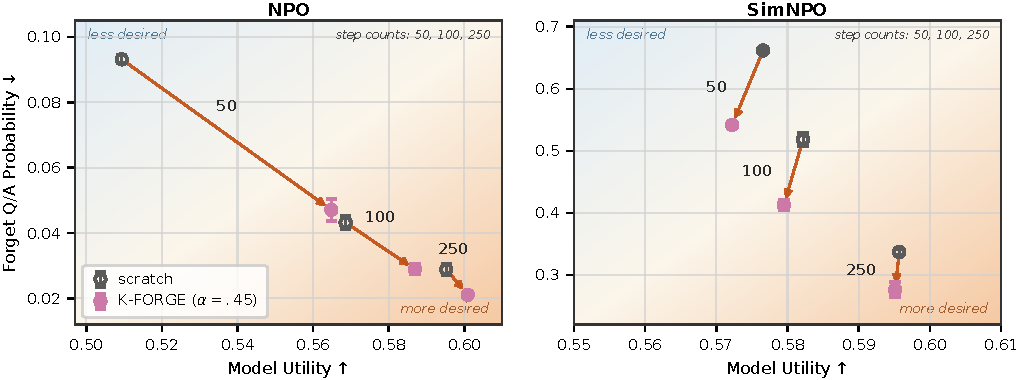
\includegraphics[width=\linewidth, trim=0cm 0.300cm 0cm 2cm]{open-unlearning/saves/figures/kforge_corrected/fig_matched_init_arrows.pdf}
    \caption{Matched downstream-step shifts on TOFU \texttt{forget10}. Arrows connect scratch runs to K-FORGE-initialized runs at the same optimizer-step budget; warmer background regions indicate higher utility and lower forget probability. Points show three-seed means with forget-probability standard deviations.}
    \label{fig:matched_init_arrows}
\end{figure*}

\subsection{K-FORGE as Initialization}
\label{sec:kforge_initialization}

After computing the low-rank edit, we form an initialized checkpoint
\begin{equation}
  \widehat{\theta}=\theta^\star + \alpha \mathbf{\Delta}^{(r)},
\end{equation}
where $\alpha$ controls edit strength. We then run an unchanged preference-based unlearning method from $\widehat{\theta}$:
\begin{equation}
  \theta_{t+1}
  =
  \theta_t - \eta_t \nabla_\theta
  \mathcal{L}_{\mathrm{unlearn}}(\theta_t),
  \qquad
  \theta_0=\widehat{\theta}.
\end{equation}
In our experiments, $\mathcal{L}_{\mathrm{unlearn}}$ is either NPO~\citep{npo} or SimNPO~\citep{simnpo}. We compare K-FORGE-initialized runs with runs started from the pretrained checkpoint.

\section{Experimental Setup}
\label{sec:experiments}

Our primary experiments use Llama-3.2-1B-Instruct. We test model-family transfer on Gemma-3-1B-IT over four seeds and report limited Llama-3.2-3B-Instruct and Qwen2.5-1.5B-Instruct checks. The MUSE experiments use Llama-2-7B. We use the OpenUnlearning training and evaluation harness~\citep{openunlearning} throughout.

\subsection{Benchmarks.}

We evaluate on TOFU~\citep{tofu}, using the \texttt{forget10}, \texttt{forget05}, and \texttt{forget01} splits, and on the News and Books domains of MUSE~\citep{muse}. The reported comparisons aggregate three seeds unless a table states otherwise; the Gemma transfer result includes a fourth seed.

\subsection{Metrics.}

Our primary endpoint is \textbf{Forget Q/A Probability}; lower values indicate less probability assigned to the gold forget answers. We also report OpenUnlearning's \textbf{Model Utility}, \textbf{Extraction Strength}, \textbf{Forget Q/A ROUGE}, \textbf{Forget Quality}, \textbf{Forget Truth Ratio}, and \textbf{PrivLeak} diagnostics. Because these metrics capture different failure modes, we report disagreements rather than combining them into one dominance claim. Reported $p$-values use two-sided paired $t$-tests; comparisons not accompanied by a $p$-value are descriptive.


\subsection{Baselines.}

Because K-FORGE is an initializer, the primary baseline is an NPO~\citep{npo} or SimNPO~\citep{simnpo} run from the pretrained checkpoint.

We also include random rank-$2$ and weight-SVD edits, a diagonal-Fisher variant related to Selective Synaptic Dampening~\citep{foster24}, and a forget-only variant. Section~\ref{sec:ablations} reports their metric-specific outcomes.

In this work, we focus on NPO and SimNPO because these preference-based unlearning methods are sensitive to initialization. RMU~\citep{rmu}, GradDiff~\citep{tofu}, and other full unlearning methods are important for the field, but including them would answer a different question: which unlearning method performs best, rather than whether K-FORGE improves a fixed downstream optimizer. We therefore treat these comparisons as outside the scope of the initializer ablation.

\subsection{K-FORGE configuration.}
Unless stated otherwise, the reported K-FORGE experiments use rank $r=2$. Tables report edit strength and downstream budget with each result.

\subsection{One-Shot K-FORGE: A Meaningful but Insufficient Forget Direction}
\label{sec:oneshot_kforge}

Table~\ref{tab:oneshot_forget10} shows the corrected one-shot frontier on TOFU \texttt{forget10}.

\begin{table}[htbp!]
\centering
\footnotesize
\setlength{\tabcolsep}{1pt}
\begin{tabular}{lcccc}
\toprule
\textbf{Method} & \textbf{Util.}$\uparrow$ & \textbf{Forget Pr.}$\downarrow$ & \textbf{ROUGE}$\downarrow$ & \textbf{Extr.}$\downarrow$ \\
\midrule
Base model & \textbf{0.599} & 0.881 & 0.820 & 0.706 \\
K-FORGE $\alpha\!=\!0.100$ & \textbf{0.599} & 0.878 & 0.814 & 0.698 \\
K-FORGE $\alpha\!=\!0.300$ & 0.595 & 0.837 & 0.721 & 0.592 \\
K-FORGE $\alpha\!=\!0.350$ & 0.594 & 0.821 & 0.692 & 0.542 \\
K-FORGE $\alpha\!=\!0.450$ & 0.582 & 0.774 & 0.613 & 0.390 \\
K-FORGE $\alpha\!=0.600$ & 0.556 & 0.657 & 0.539 & 0.262 \\
K-FORGE $\alpha\!=\!0.800$ & 0.513 & \textbf{0.411} & \textbf{0.427} & \textbf{0.130} \\
\bottomrule
\end{tabular}
\caption{One-shot results on TOFU \texttt{forget10} using Llama-3.2-1B-Instruct. We show the meaningful operating region; stronger over-edits at $\alpha\in\{1,3,10\}$ collapse utility and are reported in the released figure data rather than used as paper operating points. Best values in each metric column are bolded.}
\label{tab:oneshot_forget10}
\end{table}


The corrected frontier is smooth and interpretable: stronger edits monotonically reduce forget probability while progressively spending utility. These results support using the edit as a structured initializer rather than claiming one-shot dominance.

\section{Results}
\label{sec:results}

\begin{table*}[t]
\centering
\small
\begin{tabular}{l l l ccc}
\toprule
\textbf{Steps} & \textbf{Method} & \textbf{Init}
  & \textbf{Utility}$\uparrow$
  & \textbf{Forget Probability}$\downarrow$
  & \textbf{Extraction}$\downarrow$ \\
\midrule
\multirow{6}{*}{50}
  & \multirow{3}{*}{NPO}
  & scratch         & 0.509\stderr{0.004}          & 0.093\stderr{0.001}          & \textbf{0.068}\stderr{0.002} \\
  && K-FORGE $(0.450)$ & 0.565\stderr{0.003}          & 0.047\stderr{0.003}          & 0.072\stderr{0.003} \\
  && K-FORGE $(0.600)$ & \textbf{0.574}\stderr{0.004} & \textbf{0.045}\stderr{0.003} & 0.071\stderr{0.001} \\
\cmidrule(r){2-6}
  & \multirow{3}{*}{SimNPO}
  & scratch         & \textbf{0.577}\stderr{0.006} & 0.662\stderr{0.003}          & 0.270\stderr{0.010} \\
  && K-FORGE $(0.450)$ & 0.572\stderr{0.007}          & 0.542\stderr{0.002}          & 0.192\stderr{0.002} \\
  && K-FORGE $(0.600)$ & 0.571\stderr{0.005}          & \textbf{0.534}\stderr{0.002} & \textbf{0.188}\stderr{0.005} \\
\midrule
\multirow{6}{*}{100}
  & \multirow{3}{*}{NPO}
  & scratch         & 0.569\stderr{0.009}          & 0.043\stderr{0.002}          & \textbf{0.065}\stderr{0.003} \\
  && K-FORGE $(0.450)$ & 0.587\stderr{0.002}          & \textbf{0.029}\stderr{0.002} & 0.073\stderr{0.003} \\
  && K-FORGE $(0.600)$ & \textbf{0.593}\stderr{0.005} & 0.031\stderr{0.002}          & 0.073\stderr{0.003} \\
\cmidrule(r){2-6}
  & \multirow{3}{*}{SimNPO}
  & scratch         & \textbf{0.582}\stderr{0.002} & 0.518\stderr{0.010}          & 0.172\stderr{0.013} \\
  && K-FORGE $(0.450)$ & 0.579\stderr{0.003}          & 0.413\stderr{0.008}          & \textbf{0.143}\stderr{0.002} \\
  && K-FORGE $(0.600)$ & 0.582\stderr{0.002}          & \textbf{0.407}\stderr{0.011} & 0.144\stderr{0.005} \\
\midrule
\multirow{6}{*}{250}
  & \multirow{3}{*}{NPO}
  & scratch         & 0.595\stderr{0.009}          & 0.029\stderr{0.002}          & \textbf{0.064}\stderr{0.003} \\
  && K-FORGE $(0.450)$ & 0.601\stderr{0.003}          & \textbf{0.021}\stderr{0.001} & 0.072\stderr{0.003} \\
  && K-FORGE $(0.600)$ & \textbf{0.603}\stderr{0.004} & 0.022\stderr{0.001}          & 0.074\stderr{0.001} \\
\cmidrule(r){2-6}
  & \multirow{3}{*}{SimNPO}
  & scratch         & \textbf{0.596}\stderr{0.003} & 0.337\stderr{0.005}          & 0.116\stderr{0.004} \\
  && K-FORGE $(0.450)$ & 0.595\stderr{0.001}          & 0.276\stderr{0.012}          & 0.111\stderr{0.003} \\
  && K-FORGE $(0.600)$ & 0.592\stderr{0.004}          & \textbf{0.272}\stderr{0.008} & \textbf{0.110}\stderr{0.001} \\
\bottomrule
\end{tabular}
\caption{K-FORGE initialization ($\alpha$ value in brackets) against scratch on TOFU~\texttt{forget10}. Entries are mean $\pm$ sample standard deviation over seeds $0,1,2$ from standalone FP32 evaluation summaries.}
\label{tab:init_forget10}
\end{table*}

K-FORGE improves Forget Q/A Probability at every matched NPO budget (Table~\ref{tab:init_forget10}). The strongest effect is early: at 50 steps, the $\alpha=0.600$ initializer halves forget probability relative to scratch while improving utility by more than six points. At 250 steps, the gap narrows but remains favorable. NPO extraction is consistently higher in the K-FORGE rows, so this result supports the primary probability endpoint rather than metric-wide dominance.

SimNPO shows a smaller but more uniform relative reduction in forget probability. K-FORGE reduces forget probability at 50, 100, and 250 steps while utility remains essentially unchanged; extraction also improves at all three budgets. Thus the initializer is not tied to one preference loss: it gives NPO a large early probability gain and SimNPO a steadier gain at negligible utility cost under downstream-step matching. Section~\ref{sec:compute_overhead} separately reports setup time, FLOPs, and the slight SimNPO utility trade-off.


\subsection{Llama-3.2-3B sanity check.}
We repeat all three budgets on Llama-3.2-3B-Instruct over three seeds (Appendix Table~\ref{tab:init_3b_sanity}). SimNPO improves in utility, forget probability, extraction, and ROUGE at 50, 100, and 250 steps. NPO improves utility and forget probability strongly at 50 steps, but its forgetting metrics are worse at 100 and 250 steps. The larger-checkpoint evidence therefore supports optimizer-specific transfer rather than a general 3B claim.

\subsection{Model-family transfer.}
On Gemma-3-1B-IT, a fourth seed preserves the primary direction at $\alpha=0.800$ (Appendix Table~\ref{tab:gemma_init_controls}). Across the four same-campaign paired summaries, K-FORGE lowers NPO forget probability from 0.066 to 0.053 and extraction from 0.055 to 0.033, with similar mean utility; NPO Forget ROUGE worsens. SimNPO shows a smaller probability reduction (0.272 to 0.269) with a mean utility change of $-0.001$. This cross-family evidence is not a compute-matched comparison.


A three-seed Qwen2.5-1.5B SimNPO pilot is near-neutral: at 50 steps, scratch/K-FORGE forget probability is 0.262/0.262 and utility is 0.345/0.345; the 100-step differences are similarly negligible. We retain this null result as evidence that the initializer effect is not universal across model families.

\subsection{Transfer beyond TOFU.}
We additionally evaluate SimNPO on the News and Books domains of MUSE with Llama-2-7B (Appendix Table~\ref{tab:muse_transfer}). News provides partial transfer: at 50 steps, K-FORGE lowers both KnowMem and VerbMem forgetting scores, while extraction worsens and retain quality is nearly unchanged. At 100 steps, the follow-up improves extraction from 0.303 to 0.301 and VerbMem from 0.573 to 0.551, but not KnowMem or retain quality. Books is less favorable, with an isolated KnowMem improvement at 100 steps and adverse changes on the other metrics. MUSE therefore shows that individual forgetting gains can transfer beyond TOFU, but not a uniform benchmark-level advantage.


\subsection{Ablations}
\label{sec:ablations}
The Llama controls show that the result is not explained by inserting an arbitrary low-rank perturbation (Appendix Table~\ref{tab:init_controls_forget10}). On Llama \texttt{forget10}, K-FORGE gives the lowest forget probability among the tested initializers at the early NPO and SimNPO budgets. Thus these controls establish that data-dependent Fisher structure matters in this setting, but not that full Kronecker structure is necessary for every optimizer and metric. Appendix Table~\ref{tab:transfer_controls} reports the corresponding controls on the smaller TOFU splits.


\subsection{Robustness Audits}
\label{sec:robustness_audits}

We test active recovery through relearning and passive changes from quantized loading. For relearning, Appendix Table~\ref{tab:relearn_audit} reports scratch NPO at 100 steps and K-FORGE-initialized NPO at 50 steps before and after 13 and 39 updates.

\long\def\kforgeRelearningTable{%
\begin{table}[t]
\centering
\small
\setlength{\tabcolsep}{3pt}
\caption{Relearning trajectories over three seeds; cells are scratch/K-FORGE. Pre and 13-update values are from one-epoch runs; 39-update values are from separate three-epoch runs.}
\label{tab:relearn_audit}
\begin{tabular}{lccc}
\toprule
\textbf{Metric} & \textbf{Pre S/KF} & \textbf{Post 13 S/KF} & \textbf{Post 39 S/KF} \\
\midrule
Forget Prob. $\downarrow$ & \textbf{0.047}/0.052 & \textbf{0.376}/0.546 & \textbf{0.730}/0.911 \\
Extraction $\downarrow$ & \textbf{0.067}/0.073 & \textbf{0.112}/0.200 & \textbf{0.407}/0.812 \\
Forget ROUGE $\downarrow$ & \textbf{0.268}/0.272 & \textbf{0.376}/0.474 & \textbf{0.622}/0.884 \\
Utility $\uparrow$ & 0.568/\textbf{0.575} & 0.455/\textbf{0.493} & 0.493/\textbf{0.510} \\
\bottomrule
\end{tabular}
\end{table}
}

This does not support recovery resistance (Appendix Table~\ref{tab:relearn_audit}). After 13 updates, forget probability increases by 0.494 from K-FORGE versus 0.329 from scratch ($p<0.001$). In the separate three-epoch run, post-attack forget probability is also higher for K-FORGE (0.911 versus 0.730). SimNPO and Gemma relearning audits reach the same boundary. K-FORGE improves the pre-attack trajectory but does not prevent direct relearning.

\long\def\kforgeQuantizationTable{%
\begin{table}[t]
\centering
\small
\setlength{\tabcolsep}{4pt}
\begin{tabular}{llcccc}
\toprule
\textbf{Pair} & \textbf{Load} & \textbf{Forget Prob.}$\downarrow$ & \textbf{Utility}$\uparrow$ & \textbf{Extraction}$\downarrow$ & \textbf{ROUGE}$\downarrow$ \\
\midrule
Matched NPO & 8-bit & \textbf{0.049}/0.054 & 0.564/\textbf{0.569} & \textbf{0.066}/0.071 & \textbf{0.270}/0.275 \\
Matched NPO & 4-bit & \textbf{0.056}/0.064 & \textbf{0.531}/0.526 & \textbf{0.062}/0.065 & \textbf{0.265}/0.268 \\
SimNPO S50 & 8-bit & 0.694/\textbf{0.561} & \textbf{0.575}/0.573 & 0.284/\textbf{0.192} & 0.547/\textbf{0.465} \\
SimNPO S50 & 4-bit & 0.563/\textbf{0.472} & \textbf{0.532}/0.528 & 0.178/\textbf{0.137} & 0.468/\textbf{0.427} \\
\bottomrule
\end{tabular}
\caption{Post-quantization scratch/K-FORGE results over three paired seeds.}
\label{tab:quantization_audit}
\end{table}
}

Quantized loading is milder (Appendix Table~\ref{tab:quantization_audit}). For the NPO pair, 8-bit loading changes forget probability by $+0.002/+0.002$ from full precision and 4-bit by $+0.008/+0.012$. The SimNPO advantage persists at both precisions, but Gemma quantization erases or reverses it for NPO while preserving a small SimNPO gain. Quantization persistence is therefore optimizer-dependent and distinct from recovery resistance.

\subsection{K-FORGE compute overhead.}
\label{sec:compute_overhead}
K-FORGE adds one-time calibration, factorization, and edit cost. Table~\ref{tab:kforge_compute} reports the analytical setup estimate for one edited MLP down-projection. The edit time spans calibration through application; end-to-end also includes startup and serialization. At 1B, the complete 80.2-second setup is 40.7\%/61.5\% of evaluation-free NPO/SimNPO S50 training. FLOPs include prompt and answer tokens and exact factor rows; model passes contribute 97.7\%/99.1\% at 1B/3B. The remaining $\mathcal{O}(N(m^2+n^2)+m^3+n^3)$ factor cost limits wide or multi-layer edits.

\begin{table}[t]
\centering
\small
\setlength{\tabcolsep}{2pt}
\begin{tabular}{lcc}
\toprule
\textbf{Model} & \textbf{Edited $W$} & \textbf{Calibration} \\
 & $n{\times}m$ & ex./input tokens \\
\midrule
1B & $2048{\times}8192$ & $512/47.7\mathrm{k}$ \\
3B & $3072{\times}8192$ & $512/47.7\mathrm{k}$ \\
\bottomrule
\end{tabular}
\par\smallskip
\begin{tabular}{lccc}
\toprule
\textbf{Model} & \textbf{Time (s)} & \textbf{FLOPs} & \textbf{Eq. steps} \\
 & calib./edit/end-to-end & & NPO/SimNPO \\
\midrule
1B & $18/62/{\leq}81$ & $3.621{\times}10^{14}$ & $7.0/8.2$ \\
3B & $51/104/{\leq}145$ & $9.287{\times}10^{14}$ & $6.9/8.1$ \\
\bottomrule
\end{tabular}
\caption{One-time K-FORGE setup cost for one edited layer; analytical step equivalents include prompt and answer input tokens.}
\label{tab:kforge_compute}
\end{table}

We charge setup rather than treating it as free in the resource comparison.
For Llama-3.2-1B, the setup equals about 7.0 NPO or 8.2 SimNPO steps by FLOPs; the dynamic-padding sensitivity calculation remains below 10 steps. Table~\ref{tab:init_forget10} reports matched-step trajectories. For the strict resource audit, we charge the one-time setup to the K-FORGE S50 arm and compare it with scratch S73 for NPO and scratch S86 for SimNPO (Appendix Table~\ref{tab:kforge_compute_matched}).

\long\def\kforgeComputeMatchedTable{%
\begin{table*}[t]
\centering
\small
\setlength{\tabcolsep}{3pt}
\begin{tabular}{llrrrrrrrr}
\toprule
\textbf{Method} & \textbf{Init.} & \textbf{Steps} & \multicolumn{2}{c}{\textbf{FLOPs} ($10^{15}$)} & \textbf{Total wall} & \textbf{Forget Prob.}$\downarrow$ & \textbf{Utility}$\uparrow$ & \textbf{Extraction}$\downarrow$ & \textbf{ROUGE}$\downarrow$ \\
& & & \textbf{Train} & \textbf{Setup} & \textbf{(s)} & & & & \\
\midrule
NPO & Scratch & 73 & 3.78 & 0.00 & 285.5 & 0.059 & 0.549 & \textbf{0.067} & \textbf{0.263} \\
NPO & K-FORGE & 50 & 2.59 & 0.36 & \textbf{277.2} & \textbf{0.046} & \textbf{0.577} & 0.072 & 0.272 \\
\midrule
SimNPO & Scratch & 86 & 3.80 & 0.00 & 221.6 & 0.553 & \textbf{0.583} & 0.196 & 0.487 \\
SimNPO & K-FORGE & 50 & 2.21 & 0.36 & \textbf{210.5} & \textbf{0.537} & 0.572 & \textbf{0.188} & \textbf{0.454} \\
\bottomrule
\end{tabular}%
\caption{Independent, evaluation-free FP32 wall- and FLOP-matched TOFU \texttt{forget10} rerun over three paired seeds. Each row is a complete arm; the full 80.2-second K-FORGE setup is charged to its row.}
\label{tab:kforge_compute_matched}
\end{table*}
}

The strict comparison is strongest for NPO: K-FORGE reduces forget probability by 22.3\% ($p=0.007$, descriptive) and increases utility by 0.028 ($p<0.001$), although extraction and ROUGE worsen. SimNPO preserves the favorable probability direction in every seed and improves mean extraction and ROUGE, but the 2.8\% probability gain is descriptive ($p=0.126$) and its utility change is $-0.011$. We therefore report wall- and FLOP-matched evidence for the NPO gain, and SimNPO as a weaker trade-off rather than as a comparable-utility result.


\section{Conclusion}
\label{sec:conclusion}

We introduced \textbf{K-FORGE}, a Fisher-guided initializer with an exact full-rank Wiener solution and a stated low-rank relaxation. It improves the early Forget Q/A Probability trajectory of NPO and SimNPO on TOFU; the NPO gain remains after charging setup in FLOPs and time, while strict SimNPO matching exposes a smaller utility trade-off. Gemma provides cross-family evidence, while Qwen and MUSE show that transfer is not universal. K-FORGE is a curvature-aware starting point whose value depends on the optimizer and evaluation regime.


\section{Limitations}
\label{sec:limitations}

K-FORGE addresses initialization, not certified erasure: it requires downstream training and direct relearning recovers the forgotten behavior. Evidence is strongest for Forget Q/A Probability on TOFU; NPO extraction, Forget ROUGE, and MUSE can disagree, and transfer is uneven across model families. For one 1B layer, complete setup costs 40.7\% of an evaluation-free NPO S50 run and 61.5\% of a SimNPO S50 run by wall-clock time, versus 14.0\% and 16.4\% by analytical FLOPs. Multi-layer and broader large-model scaling remain open.

% Bibliography entries for the entire Anthology, followed by custom entries
%\bibliography{anthology,custom}
% Custom bibliography entries only
\bibliography{custom}
\onecolumn
\long\def\kforgeAppendixResults{%
\section{Additional Experimental Results}
\label{sec:appendix_results}

\begin{table}[htbp!]
\centering
\small
\begin{tabular}{l l cccc}
\toprule
\multicolumn{1}{c}{\textbf{Method}}
  & \multicolumn{1}{l}{\textbf{Init}}
  & \multicolumn{2}{c}{\textbf{S50}}
  & \multicolumn{2}{c}{\textbf{S100}} \\
\cmidrule(lr){3-4}\cmidrule(lr){5-6}
& & \textbf{Utility}$\uparrow$ & \textbf{Forget Pr.}$\downarrow$
    & \textbf{Utility}$\uparrow$ & \textbf{Forget Pr.}$\downarrow$ \\
\midrule
\multirow{6}{*}[-0.200em]{NPO}
 & scratch           & 0.509\stderr{0.004} & 0.093\stderr{0.001} & 0.569\stderr{0.009} & 0.043\stderr{0.002} \\
 & random            & 0.516\stderr{0.004} & 0.082\stderr{0.005} & 0.579\stderr{0.008} & 0.038\stderr{0.005} \\
 & weight-SVD              & 0.538\stderr{0.012} & 0.084\stderr{0.006} & \textbf{0.587}\stderr{0.003} & 0.043\stderr{0.001} \\
 & diagonal          & 0.561\stderr{0.007} & 0.058\stderr{0.007} & 0.584\stderr{0.011} & 0.033\stderr{0.001} \\
 & forget-only       & 0.543\stderr{0.004} & 0.062\stderr{0.004} & 0.582\stderr{0.003} & 0.032\stderr{0.001} \\
 & \textbf{K-FORGE}  & \textbf{0.565}\stderr{0.003} & \textbf{0.047}\stderr{0.003} & \textbf{0.587}\stderr{0.002} & \textbf{0.029}\stderr{0.002} \\
\cmidrule{2-6}
\multirow{6}{*}[-0.200em]{SimNPO}
 & scratch           & 0.577\stderr{0.006} & 0.662\stderr{0.003} & 0.582\stderr{0.002} & 0.518\stderr{0.010} \\
 & random            & \textbf{0.578}\stderr{0.011} & 0.650\stderr{0.004} & 0.584\stderr{0.001} & 0.515\stderr{0.002} \\
 & weight-SVD              & 0.574\stderr{0.005} & 0.619\stderr{0.006} & \textbf{0.585}\stderr{0.003} & 0.488\stderr{0.005} \\
 & diagonal          & 0.570\stderr{0.003} & 0.607\stderr{0.002} & 0.583\stderr{0.003} & 0.500\stderr{0.007} \\
 & forget-only       & 0.572\stderr{0.005} & 0.619\stderr{0.006} & 0.583\stderr{0.001} & 0.491\stderr{0.004} \\
 & \textbf{K-FORGE}  & 0.572\stderr{0.007} & \textbf{0.542}\stderr{0.002} & 0.579\stderr{0.003} & \textbf{0.413}\stderr{0.008} \\
\bottomrule
\end{tabular}
\caption{Initialization controls on TOFU \texttt{forget10}. Best values are bolded within each method and step-budget block.}
\label{tab:init_controls_forget10}
\end{table}

\begin{table}[htbp!]
\centering
\small
\setlength{\tabcolsep}{4pt}
\begin{tabular}{rllcccc}
\toprule
\textbf{Steps} & \textbf{Method} & \textbf{Init.} & \textbf{Util.}$\uparrow$ & \textbf{Forget Pr.}$\downarrow$ & \textbf{Extr.}$\downarrow$ & \textbf{ROUGE}$\downarrow$ \\
\midrule
\multirow{4}{*}{50}
  & \multirow{2}{*}{NPO}
  & scratch & 0.589\stderr{0.021} & 0.086\stderr{0.005} & \textbf{0.057}\stderr{0.006} & \textbf{0.237}\stderr{0.010} \\
  && K-FORGE & \textbf{0.639}\stderr{0.015} & \textbf{0.065}\stderr{0.004} & 0.070\stderr{0.001} & 0.293\stderr{0.005} \\
\cmidrule(r){2-7}
  & \multirow{2}{*}{SimNPO}
  & scratch & 0.636\stderr{0.005} & 0.691\stderr{0.008} & 0.351\stderr{0.007} & 0.587\stderr{0.006} \\
  && K-FORGE & \textbf{0.656}\stderr{0.009} & \textbf{0.583}\stderr{0.004} & \textbf{0.264}\stderr{0.006} & \textbf{0.519}\stderr{0.008} \\
\midrule
\multirow{4}{*}{100}
  & \multirow{2}{*}{NPO}
  & scratch & 0.648\stderr{0.024} & \textbf{0.034}\stderr{0.003} & \textbf{0.055}\stderr{0.004} & \textbf{0.260}\stderr{0.012} \\
  && K-FORGE & \textbf{0.670}\stderr{0.006} & 0.039\stderr{0.002} & 0.077\stderr{0.001} & 0.306\stderr{0.010} \\
\cmidrule(r){2-7}
  & \multirow{2}{*}{SimNPO}
  & scratch & 0.647\stderr{0.009} & 0.517\stderr{0.006} & 0.223\stderr{0.005} & 0.486\stderr{0.004} \\
  && K-FORGE & \textbf{0.655}\stderr{0.003} & \textbf{0.455}\stderr{0.006} & \textbf{0.191}\stderr{0.005} & \textbf{0.467}\stderr{0.004} \\
\midrule
\multirow{4}{*}{250}
  & \multirow{2}{*}{NPO}
  & scratch & \textbf{0.665}\stderr{0.008} & \textbf{0.027}\stderr{0.003} & \textbf{0.057}\stderr{0.003} & \textbf{0.261}\stderr{0.007} \\
  && K-FORGE & 0.662\stderr{0.008} & 0.029\stderr{0.001} & 0.079\stderr{0.002} & 0.302\stderr{0.008} \\
\cmidrule(r){2-7}
  & \multirow{2}{*}{SimNPO}
  & scratch & 0.662\stderr{0.005} & 0.334\stderr{0.002} & 0.151\stderr{0.001} & 0.434\stderr{0.009} \\
  && K-FORGE & \textbf{0.666}\stderr{0.007} & \textbf{0.314}\stderr{0.005} & \textbf{0.142}\stderr{0.002} & \textbf{0.429}\stderr{0.008} \\
\bottomrule
\end{tabular}
\caption{Three-seed Llama-3.2-3B-Instruct results on TOFU \texttt{forget10}. K-FORGE uses $\alpha=0.450$; best values are bolded within each method and budget.}
\label{tab:init_3b_sanity}
\end{table}

\begin{table}[htbp!]
\centering
\small
\begin{tabular}{lllcccc}
\toprule
\multicolumn{1}{c}{\textbf{Split}}
  & \multicolumn{1}{c}{\textbf{Method}}
  & \multicolumn{1}{c}{\textbf{Init}}
  & \multicolumn{2}{c}{\textbf{S50}}
  & \multicolumn{2}{c}{\textbf{S100}} \\
\cmidrule(lr){4-5}\cmidrule(lr){6-7}
& & & \textbf{Utility}$\uparrow$ & \textbf{Forget Pr.}$\downarrow$
    & \textbf{Utility}$\uparrow$ & \textbf{Forget Pr.}$\downarrow$ \\
\midrule
\multirow{8}{*}[-0.200em]{\texttt{f01}}
 & \multirow{4}{*}[-0.200em]{NPO}
 & scratch      & \textbf{0.578}\stderr{0.003} & 0.014\stderr{0.001} & 0.580\stderr{0.000} & 0.012\stderr{0.001} \\
 & & random       & 0.574\stderr{0.003} & 0.013\stderr{0.002} & 0.579\stderr{0.001} & 0.012\stderr{0.002} \\
 & & weight-SVD   & 0.577\stderr{0.002} & 0.013\stderr{0.002} & \textbf{0.582}\stderr{0.001} & 0.012\stderr{0.001} \\
 & & K-FORGE      & 0.573\stderr{0.001} & \textbf{0.010}\stderr{0.001} & 0.579\stderr{0.004} & \textbf{0.011}\stderr{0.001} \\
\cmidrule(r){3-7}
 & \multirow{4}{*}[-0.200em]{SimNPO}
 & scratch      & 0.573\stderr{0.008} & 0.288\stderr{0.005} & \textbf{0.580}\stderr{0.008} & 0.242\stderr{0.008} \\
 & & random       & 0.573\stderr{0.007} & 0.286\stderr{0.006} & \textbf{0.580}\stderr{0.006} & 0.241\stderr{0.010} \\
 & & weight-SVD   & \textbf{0.575}\stderr{0.006} & 0.304\stderr{0.007} & 0.578\stderr{0.007} & 0.256\stderr{0.014} \\
 & & K-FORGE     & 0.570\stderr{0.008} & \textbf{0.238}\stderr{0.008} & 0.577\stderr{0.007} & \textbf{0.209}\stderr{0.005} \\
\midrule
\multirow{7}{*}[-0.200em]{\texttt{f05}}
 & \multirow{4}{*}[-0.200em]{NPO}
 & scratch      & 0.542\stderr{0.007} & 0.050\stderr{0.005} & 0.578\stderr{0.009} & 0.028\stderr{0.001} \\
 & & random       & 0.557\stderr{0.005} & 0.043\stderr{0.006} & 0.580\stderr{0.002} & \textbf{0.025}\stderr{0.002} \\
 & & weight-SVD   & 0.573\stderr{0.007} & 0.043\stderr{0.003} & \textbf{0.592}\stderr{0.002} & 0.034\stderr{0.002} \\
 & & K-FORGE      & \textbf{0.575}\stderr{0.003} & \textbf{0.032}\stderr{0.002} & 0.586\stderr{0.005} & \textbf{0.025}\stderr{0.001} \\
\cmidrule(r){3-7}
 & \multirow{3}{*}[-0.200em]{SimNPO}
 & scratch      & 0.573\stderr{0.010} & 0.549\stderr{0.029} & 0.586\stderr{0.001} & 0.417\stderr{0.016} \\
 & & weight-SVD   & \textbf{0.575}\stderr{0.007} & 0.476\stderr{0.010} & \textbf{0.588}\stderr{0.003} & 0.375\stderr{0.005} \\
 & & K-FORGE      & 0.571\stderr{0.004} & \textbf{0.425}\stderr{0.012} & 0.586\stderr{0.005} & \textbf{0.331}\stderr{0.010} \\
\bottomrule
\end{tabular}
\caption{Transfer initialization controls on TOFU splits \texttt{forget05} and \texttt{forget01} (denoted as \texttt{f05} and \texttt{f01}). Best values are bolded within each split, method, and step-budget block.}
\label{tab:transfer_controls}
\end{table}



\begin{table}[htbp!]
\centering
\small
\setlength{\tabcolsep}{4pt}
\begin{tabular}{lllrlll}
\toprule
\textbf{Domain} & \textbf{Steps} & \textbf{Init.} & \textbf{Extr.}$\downarrow$ & \textbf{KnowMem}$\downarrow$ & \textbf{VerbMem}$\downarrow$ & \textbf{Retain}$\uparrow$ \\
\midrule
\multirow{5}{*}{News}
 & 50 & scratch & \textbf{0.307}\stderr{0.002} & 0.630\stderr{0.006} & 0.574\stderr{0.002} & \textbf{0.534}\stderr{0.007} \\
 & 50 & K-FORGE & 0.315\stderr{0.004} & \textbf{0.624}\stderr{0.010} & \textbf{0.564}\stderr{0.012} & 0.532\stderr{0.006} \\
 & 100 & scratch & 0.303\stderr{0.004} & 0.629\stderr{0.002} & 0.573\stderr{0.003} & \textbf{0.532}\stderr{0.008} \\
 & 100 & K-FORGE $(0.450)$ & 0.310\stderr{0.001} & \textbf{0.628}\stderr{0.006} & 0.562\stderr{0.012} & 0.522\stderr{0.006} \\
 & 100 & K-FORGE $(1.000)$ & \textbf{0.301}\stderr{0.000} & 0.629\stderr{0.007} & \textbf{0.551}\stderr{0.007} & 0.520\stderr{0.011} \\
\midrule
\multirow{4}{*}{Books}
 & 50 & scratch & 0.911\stderr{0.000} & \textbf{0.411}\stderr{0.013} & \textbf{0.994}\stderr{0.005} & \textbf{0.649}\stderr{0.001} \\
 & 50 & K-FORGE & \textbf{0.911}\stderr{0.000} & 0.426\stderr{0.005} & 0.996\stderr{0.002} & 0.645\stderr{0.006} \\
 & 100 & scratch & \textbf{0.852}\stderr{0.025} & 0.365\stderr{0.010} & \textbf{0.955}\stderr{0.020} & \textbf{0.610}\stderr{0.006} \\
 & 100 & K-FORGE & 0.869\stderr{0.020} & \textbf{0.357}\stderr{0.002} & 0.963\stderr{0.013} & 0.586\stderr{0.017} \\
\bottomrule
\end{tabular}
\caption{Three-seed MUSE transfer with SimNPO and Llama-2-7B. K-FORGE uses $\alpha=0.450$ unless shown otherwise.}
\label{tab:muse_transfer}
\end{table}

\begin{table}[htbp!]
\centering
\small
\setlength{\tabcolsep}{3pt}
\begin{tabular}{llcccc}
\toprule
\textbf{Method} & \textbf{Init.} & \textbf{Utility}$\uparrow$ & \textbf{Forget Pr.}$\downarrow$ & \textbf{Extr.}$\downarrow$ & \textbf{ROUGE}$\downarrow$ \\
\midrule
\multirow{2}{*}{NPO}
 & scratch & 0.401\stderr{0.002} & 0.066\stderr{0.002} & 0.055\stderr{0.004} & \textbf{0.298}\stderr{0.013} \\
 & K-FORGE & \textbf{0.401}\stderr{0.013} & 0.053\stderr{0.003} & \textbf{0.033}\stderr{0.002} & 0.365\stderr{0.009} \\
\midrule
\multirow{2}{*}{SimNPO}
 & scratch & 0.410\stderr{0.002} & 0.272\stderr{0.000} & 0.127\stderr{0.003} & 0.399\stderr{0.004} \\
 & K-FORGE & 0.409\stderr{0.002} & 0.269\stderr{0.000} & \textbf{0.122}\stderr{0.001} & \textbf{0.395}\stderr{0.005} \\
\bottomrule
\end{tabular}
\caption{Four-seed same-campaign Gemma-3-1B comparison at 100 downstream steps. Best means are bolded within each optimizer.}
\label{tab:gemma_init_controls}
\end{table}

\begin{table}[htbp!]
\centering
\small
\setlength{\tabcolsep}{4pt}
\begin{tabular}{rllcccc}
\toprule
\textbf{Steps} & \textbf{Init.} & \textbf{$n$} & \textbf{Utility}$\uparrow$ & \textbf{Forget Pr.}$\downarrow$ & \textbf{Extr.}$\downarrow$ & \textbf{ROUGE}$\downarrow$ \\
\midrule
50 & scratch & 3 & \textbf{0.345}\stderr{0.002} & 0.262\stderr{0.000} & \textbf{0.121}\stderr{0.001} & 0.359\stderr{0.004} \\
50 & K-FORGE & 3 & 0.345\stderr{0.002} & \textbf{0.262}\stderr{0.000} & 0.121\stderr{0.001} & \textbf{0.356}\stderr{0.003} \\
\midrule
100 & scratch & 3 & 0.345\stderr{0.000} & 0.262\stderr{0.000} & \textbf{0.120}\stderr{0.001} & 0.361\stderr{0.004} \\
100 & K-FORGE & 3 & \textbf{0.345}\stderr{0.000} & \textbf{0.262}\stderr{0.000} & 0.121\stderr{0.001} & \textbf{0.360}\stderr{0.004} \\
\bottomrule
\end{tabular}
\caption{Three-seed Qwen2.5-1.5B SimNPO pilot on TOFU \texttt{forget10}. K-FORGE edits layer 15 with rank $2$ and $\alpha=0.450$.}
\label{tab:qwen_pilot}
\end{table}

\kforgeComputeMatchedTable
\kforgeRelearningTable
\kforgeQuantizationTable

\begin{table}[htbp!]
\centering
\small
\setlength{\tabcolsep}{6pt}
\begin{tabular}{llrlrrrr}
\toprule
\textbf{Model} & \textbf{Method} & \textbf{Updates} & \textbf{Init.} & \textbf{FP}$\downarrow$ & \textbf{Utility}$\uparrow$ & \textbf{Extr.}$\downarrow$ & \textbf{ROUGE}$\downarrow$ \\
\midrule
\multirow{6}{*}{Llama-1B} & \multirow{6}{*}{SimNPO}
 & \multirow{2}{*}{0} & scratch & \textbf{0.545} & \textbf{0.585} & \textbf{0.184} & 0.480 \\
 & & & K-FORGE & 0.569 & 0.575 & 0.202 & \textbf{0.466} \\
 & & \multirow{2}{*}{13} & scratch & \textbf{0.803} & 0.560 & \textbf{0.539} & \textbf{0.708} \\
 & & & K-FORGE & 0.874 & \textbf{0.564} & 0.694 & 0.815 \\
 & & \multirow{2}{*}{39} & scratch & \textbf{0.978} & \textbf{0.565} & \textbf{0.968} & \textbf{0.984} \\
 & & & K-FORGE & 0.982 & 0.553 & 0.977 & 0.987 \\
\midrule
\multirow{6}{*}{Gemma-1B} & \multirow{6}{*}{NPO}
 & \multirow{2}{*}{0} & scratch & 0.074 & 0.350 & 0.031 & \textbf{0.318} \\
 & & & K-FORGE & \textbf{0.074} & \textbf{0.357} & \textbf{0.030} & 0.383 \\
 & & \multirow{2}{*}{13} & scratch & \textbf{0.261} & 0.352 & \textbf{0.119} & \textbf{0.414} \\
 & & & K-FORGE & 0.295 & \textbf{0.374} & 0.135 & 0.415 \\
 & & \multirow{2}{*}{39} & scratch & \textbf{0.501} & \textbf{0.395} & \textbf{0.197} & \textbf{0.490} \\
 & & & K-FORGE & 0.552 & 0.394 & 0.225 & 0.520 \\
\midrule
\multirow{6}{*}{Gemma-1B} & \multirow{6}{*}{SimNPO}
 & \multirow{2}{*}{0} & scratch & 0.273 & \textbf{0.404} & 0.127 & 0.406 \\
 & & & K-FORGE & \textbf{0.270} & 0.403 & \textbf{0.122} & \textbf{0.402} \\
 & & \multirow{2}{*}{13} & scratch & \textbf{0.353} & 0.385 & 0.145 & 0.436 \\
 & & & K-FORGE & 0.353 & \textbf{0.385} & \textbf{0.145} & \textbf{0.433} \\
 & & \multirow{2}{*}{39} & scratch & \textbf{0.658} & \textbf{0.396} & \textbf{0.283} & \textbf{0.597} \\
 & & & K-FORGE & 0.665 & 0.393 & 0.296 & 0.598 \\
\bottomrule
\end{tabular}%
\caption{Additional relearning trajectories over three seeds. Update 0 is the pre-attack operating point.}
\label{tab:additional_relearning}
\end{table}

\begin{table}[htbp!]
\centering
\small
\setlength{\tabcolsep}{4pt}
\begin{tabular}{lllrlll}
\toprule
\textbf{Method} & \textbf{Load} & \textbf{Init.} & \textbf{Forget Pr.}$\downarrow$ & \textbf{Utility}$\uparrow$ & \textbf{Extr.}$\downarrow$ & \textbf{ROUGE}$\downarrow$ \\
\midrule
\multirow{4}{*}{NPO}
 & 8-bit & scratch & 0.070 & 0.388 & 0.053 & \textbf{0.302} \\
 & 8-bit & K-FORGE & \textbf{0.070} & \textbf{0.390} & \textbf{0.034} & 0.368 \\
 & 4-bit & scratch & \textbf{0.058} & \textbf{0.327} & 0.035 & \textbf{0.330} \\
 & 4-bit & K-FORGE & 0.061 & 0.295 & \textbf{0.030} & 0.399 \\
\midrule
\multirow{4}{*}{SimNPO}
 & 8-bit & scratch & 0.269 & \textbf{0.403} & 0.123 & 0.402 \\
 & 8-bit & K-FORGE & \textbf{0.266} & 0.403 & \textbf{0.121} & \textbf{0.402} \\
 & 4-bit & scratch & 0.219 & 0.388 & 0.102 & 0.419 \\
 & 4-bit & K-FORGE & \textbf{0.214} & \textbf{0.390} & \textbf{0.101} & \textbf{0.417} \\
\bottomrule
\end{tabular}
\caption{Four-seed Gemma-3-1B results after 8-bit and 4-bit loading. Best means are bolded within each method and precision.}
\label{tab:gemma_quantization}
\end{table}

}

\appendix
\section{Proofs}
\label{sec:proofs}

Throughout this appendix we use the notation of Section~\ref{sec:method}. Let $\mathbf{W}\in\mathbb{R}^{n\times m}$, $\mathbf{A}_\bullet\in\mathbb{R}^{m\times m}$, $\mathbf{B}_\bullet\in\mathbb{R}^{n\times n}$, with Cholesky factors $\mathbf{L}_{A_\bullet}$, $\mathbf{L}_{B_\bullet}$ and cross-Cholesky SVDs
\begin{align*}
\mathbf{K}_A &= \mathbf{L}_{A_r}^{-1}\mathbf{L}_{A_f} = \mathbf{U}_A\mathbf{\Sigma}_A\mathbf{V}_A^\top, \\
\mathbf{K}_B &= \mathbf{L}_{B_r}^{-1}\mathbf{L}_{B_f} = \mathbf{U}_B\mathbf{\Sigma}_B\mathbf{V}_B^\top.
\end{align*}
The simultaneous diagonalizers are $\mathbf{Q}_A = \mathbf{L}_{A_r}^{-\top}\mathbf{U}_A$ and $\mathbf{Q}_B = \mathbf{L}_{B_r}^{-\top}\mathbf{U}_B$. Standard algebra gives $\mathbf{Q}_A^\top\mathbf{A}_f\mathbf{Q}_A = \mathbf{\Sigma}_A^2$, $\mathbf{Q}_A^\top\mathbf{A}_r\mathbf{Q}_A = \mathbf{I}$, and analogously for $\mathbf{Q}_B$. We parametrize the perturbation as $\mathbf{\Delta} = \mathbf{Q}_B\mathbf{H}\mathbf{Q}_A^\top$ with $\mathbf{H}\in\mathbb{R}^{n\times m}$.

\subsection{Lemma: change of coordinates}
\label{app:coordlemma}

\begin{lemma}
\label{lem:coords}
Let $\mathbf{M} := \mathbf{Q}_B^{-1}\mathbf{W}\mathbf{Q}_A^{-\top}$. Then
\[
J(\mathbf{\Delta}) = \sum_{j,i}\Big[\sigma_{A,i}^2\sigma_{B,j}^2(M_{ji}+H_{ji})^2 + \lambda_{\mathrm{ret}} H_{ji}^2\Big],
\]
and $\mathbf{M} = \mathbf{\Sigma}_B^{-1}\mathbf{R}\mathbf{\Sigma}_A^{-1}$, where $\mathbf{R} = \mathbf{V}_B^\top\mathbf{L}_{B_f}^\top\mathbf{W}\mathbf{L}_{A_f}\mathbf{V}_A$.
\end{lemma}

\begin{proof}
By definition of $\mathbf{M}$, $\mathbf{W} = \mathbf{Q}_B\mathbf{M}\mathbf{Q}_A^\top$, so $\mathbf{W}+\mathbf{\Delta} = \mathbf{Q}_B(\mathbf{M}+\mathbf{H})\mathbf{Q}_A^\top$. Using $\operatorname{vec}(\mathbf{Q}_B\mathbf{X}\mathbf{Q}_A^\top) = (\mathbf{Q}_A\otimes\mathbf{Q}_B)\operatorname{vec}(\mathbf{X})$ and the diagonalizing identities,
\begin{equation}
\lVert\mathbf{W}+\mathbf{\Delta}\rVert^2_{F_f}=
\operatorname{vec}(\mathbf{M}+\mathbf{H})^\top
\bigl(\mathbf{\Sigma}_A^2\otimes\mathbf{\Sigma}_B^2\bigr)\operatorname{vec}(\mathbf{M}+\mathbf{H}) =\sum_{j,i}
\sigma_{A,i}^2\sigma_{B,j}^2
(M_{ji}+H_{ji})^2 .
\end{equation}
and analogously $\lVert\mathbf{\Delta}\rVert^2_{F_r} = \lVert\mathbf{H}\rVert_F^2$.

For the second claim, $\mathbf{K}_B = \mathbf{L}_{B_r}^{-1}\mathbf{L}_{B_f}$ gives $\mathbf{L}_{B_r}\mathbf{U}_B = \mathbf{L}_{B_f}\mathbf{V}_B\mathbf{\Sigma}_B^{-1}$, hence $\mathbf{L}_{B_r} = \mathbf{L}_{B_f}\mathbf{V}_B\mathbf{\Sigma}_B^{-1}\mathbf{U}_B^\top$ and $\mathbf{U}_B^\top\mathbf{L}_{B_r}^\top = \mathbf{\Sigma}_B^{-1}\mathbf{V}_B^\top\mathbf{L}_{B_f}^\top$. By analogous algebra, $\mathbf{L}_{A_r}\mathbf{U}_A = \mathbf{L}_{A_f}\mathbf{V}_A\mathbf{\Sigma}_A^{-1}$. Therefore
\begin{align*}
\mathbf{M} &= \mathbf{Q}_B^{-1}\mathbf{W}\mathbf{Q}_A^{-\top} = \mathbf{U}_B^\top\mathbf{L}_{B_r}^\top\mathbf{W}\mathbf{L}_{A_r}\mathbf{U}_A \\
&= \mathbf{\Sigma}_B^{-1}\mathbf{V}_B^\top\mathbf{L}_{B_f}^\top\mathbf{W}\mathbf{L}_{A_f}\mathbf{V}_A\mathbf{\Sigma}_A^{-1} \\
&= \mathbf{\Sigma}_B^{-1}\mathbf{R}\mathbf{\Sigma}_A^{-1}. \qedhere
\end{align*}
\end{proof}

\subsection{Proof of Theorem~\ref{thm:two_fisher_gsvd}}
\label{app:thm_proof}

\begin{proof}
By Lemma~\ref{lem:coords}, $J$ is separable across entries $(j,i)$, so its Hessian in $\mathbf{H}$ is diagonal with entries $2(\sigma_{A,i}^2\sigma_{B,j}^2 + \lambda_{\mathrm{ret}})$. Under the assumption $\sigma_{A,i},\sigma_{B,j}>0$ (Section~\ref{sec:preliminaries}), each entry is strictly positive, so $J$ is strictly convex and admits a unique minimizer. Setting the partial derivative to zero,
\[
2\sigma_{A,i}^2\sigma_{B,j}^2(M_{ji}+H_{ji}) + 2\lambda_{\mathrm{ret}}H_{ji} = 0,
\]
yields
\[
H_{ji}^\star = -\frac{\sigma_{A,i}^2\sigma_{B,j}^2}{\sigma_{A,i}^2\sigma_{B,j}^2 + \lambda_{\mathrm{ret}}}\,M_{ji}.
\]
Substituting $M_{ji} = R_{ji}/(\sigma_{A,i}\sigma_{B,j})$ from Lemma~\ref{lem:coords},
\[
H_{ji}^\star = -\frac{\sigma_{A,i}\sigma_{B,j}}{\sigma_{A,i}^2\sigma_{B,j}^2 + \lambda_{\mathrm{ret}}}\,R_{ji} = -G_{ji}R_{ji},
\]
so $\mathbf{H}^\star = -(\mathbf{G}\odot\mathbf{R})$. Mapping back,
\[
\mathbf{\Delta}^\star = \mathbf{Q}_B\mathbf{H}^\star\mathbf{Q}_A^\top = -\mathbf{L}_{B_r}^{-\top}\mathbf{U}_B(\mathbf{G}\odot\mathbf{R})\mathbf{U}_A^\top\mathbf{L}_{A_r}^{-1}.
\]
For $r=\min(m,n)$ the rank constraint is inactive, so $\mathbf{\Delta}^\star$ is also the rank-$r$ minimizer.
\end{proof}

\subsection{Proof of Proposition~\ref{prop:rankr_lam0}}
\label{app:prop1_proof}

\begin{proof}
Set $\lambda_{\mathrm{ret}}=0$. By Lemma~\ref{lem:coords},
\[
J(\mathbf{\Delta})\big|_{\lambda=0}
= \sum_{j,i}\sigma_{A,i}^2\sigma_{B,j}^2(M_{ji}+H_{ji})^2
= \lVert\mathbf{\Sigma}_B(\mathbf{M}+\mathbf{H})\mathbf{\Sigma}_A\rVert_F^2.
\]


Using $\mathbf{\Sigma}_B\mathbf{M}\mathbf{\Sigma}_A = \mathbf{R}$ and defining $\mathbf{Y} := \mathbf{\Sigma}_B\mathbf{H}\mathbf{\Sigma}_A$,
\[
J|_{\lambda=0}(\mathbf{H}) = \lVert\mathbf{Y}+\mathbf{R}\rVert_F^2.
\]
Since $\mathbf{\Sigma}_A,\mathbf{\Sigma}_B$ are invertible diagonal and $\mathbf{Q}_A,\mathbf{Q}_B$ are invertible, $\operatorname{rank}(\mathbf{\Delta})\le r \Leftrightarrow \operatorname{rank}(\mathbf{H})\le r \Leftrightarrow \operatorname{rank}(\mathbf{Y})\le r$. The constrained problem becomes
\[
\min_{\operatorname{rank}(\mathbf{Y})\le r}\lVert\mathbf{Y} - (-\mathbf{R})\rVert_F^2,
\]
whose Eckart--Young (Frobenius) minimizer may be chosen as $\mathbf{Y}_r=-\operatorname{SVD}_r(\mathbf{R})$; equivalently, any rank-$r$ SVD truncation of $-\mathbf{R}$ attains the optimum. The minimizer is unique when $\sigma_r(\mathbf{R}) > \sigma_{r+1}(\mathbf{R})$. Unscaling this choice gives $\mathbf{H}_r = -\mathbf{\Sigma}_B^{-1}\operatorname{SVD}_r(\mathbf{R})\mathbf{\Sigma}_A^{-1}$, and
\[
\mathbf{\Delta}^{(r)}_{\lambda=0} = \mathbf{Q}_B\mathbf{H}_r\mathbf{Q}_A^\top = -\mathbf{L}_{B_r}^{-\top}\mathbf{U}_B\mathbf{\Sigma}_B^{-1}\operatorname{SVD}_r(\mathbf{R})\mathbf{\Sigma}_A^{-1}\mathbf{U}_A^\top\mathbf{L}_{A_r}^{-1}. \qedhere
\]
\end{proof}

\subsection{Proposition~\ref{prop:limit_consistency}: Limit consistency of the relaxation.}

\begin{proposition}
\label{prop:limit_consistency}
The relaxed edit $\mathbf{\Delta}^{(r)}$ in Eq.~\ref{eq:kforge_relaxed_delta} is exact in two limits: (i) at $r=\min(m,n)$ it equals the unique minimizer $\mathbf{\Delta}^\star$ from Theorem~\ref{thm:two_fisher_gsvd} for any $\lambda_{\mathrm{ret}}\ge 0$; (ii) at $\lambda_{\mathrm{ret}}=0$ it equals an exact rank-$r$ minimizer from Proposition~\ref{prop:rankr_lam0} for any $r$.
\end{proposition}

\begin{proof}
\emph{Case (i): $r = \min(m,n)$.} The truncation $\operatorname{SVD}_r(\mathbf{Y}^\star) = \mathbf{Y}^\star$ is vacuous, so $\mathbf{H}_r = \mathbf{\Sigma}_B^{-1}\mathbf{Y}^\star\mathbf{\Sigma}_A^{-1} = -\mathbf{\Sigma}_B^{-1}(\widetilde{\mathbf{G}}\odot\mathbf{R})\mathbf{\Sigma}_A^{-1}$. Entrywise,
\[
(H_r)_{ji} = -\frac{\widetilde{G}_{ji}}{\sigma_{A,i}\sigma_{B,j}}R_{ji}
= -\frac{\sigma_{A,i}\sigma_{B,j}}{\sigma_{A,i}^2\sigma_{B,j}^2+\lambda_{\mathrm{ret}}}R_{ji}
= -G_{ji}R_{ji},
\]
which is $\mathbf{H}^\star$ from the proof of Theorem~\ref{thm:two_fisher_gsvd}. Hence $\mathbf{\Delta}^{(r)} = \mathbf{Q}_B\mathbf{H}^\star\mathbf{Q}_A^\top = \mathbf{\Delta}^\star$.

\emph{Case (ii): $\lambda_{\mathrm{ret}} = 0$.} Then


$$  
\widetilde{G}_{ji} = \frac{\sigma_{A,i}^2\sigma_{B,j}^2}{ \sigma_{A,i}^2\sigma_{B,j}^2} = 1.
$$ 

Thus $\mathbf{Y}^\star = -\mathbf{R}$, and any
$\mathbf{Y}_r=\operatorname{SVD}_r(-\mathbf{R})$ is an Eckart--Young
minimizer of the transformed problem. Unscaling
$\mathbf{H}_r=\mathbf{\Sigma}_B^{-1}\mathbf{Y}_r\mathbf{\Sigma}_A^{-1}$
and mapping back
$\mathbf{\Delta}^{(r)}=\mathbf{Q}_B\mathbf{H}_r\mathbf{Q}_A^\top$
therefore yields an exact rank-$r$ minimizer characterized by
Proposition~\ref{prop:rankr_lam0}.
\end{proof}

% Keep the experimental appendix separate from the final proof and top-align table-only pages.
\clearpage
\makeatletter
\setlength{\@fptop}{0pt}
\setlength{\@fpsep}{12pt}
\makeatother
\kforgeAppendixResults

\end{document}
